% Appendix A

\chapter{More Visualization} % Main appendix title

\label{AppendixB} % For referencing this appendix elsewhere, use \ref{AppendixA}

%% gcnn-Visual-more
\newpage
\begin{figure}
	\centering
	\captionsetup{width=\linewidth}
	\begin{subfigure}[b]{0.24\linewidth}
		
\includegraphics[width=\linewidth]{./Figures/gcnn_synthetic/fancy_eval_2_point_cloud_noise.png}
	\end{subfigure}
	\begin{subfigure}[b]{0.24\linewidth}
		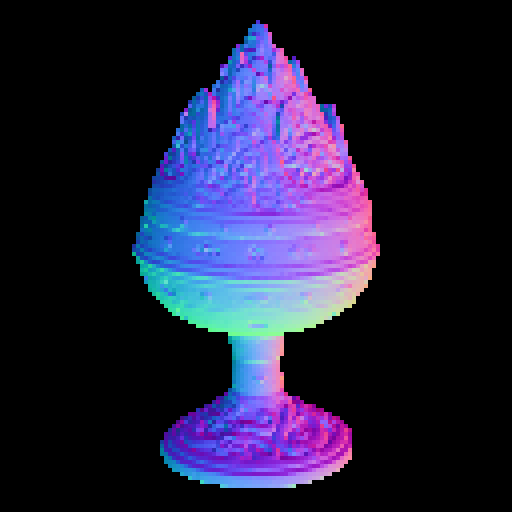
\includegraphics[width=\linewidth]{./Figures/gcnn_synthetic/fancy_eval_2_groundtruth.png}
	\end{subfigure}
	\begin{subfigure}[b]{0.24\linewidth}
		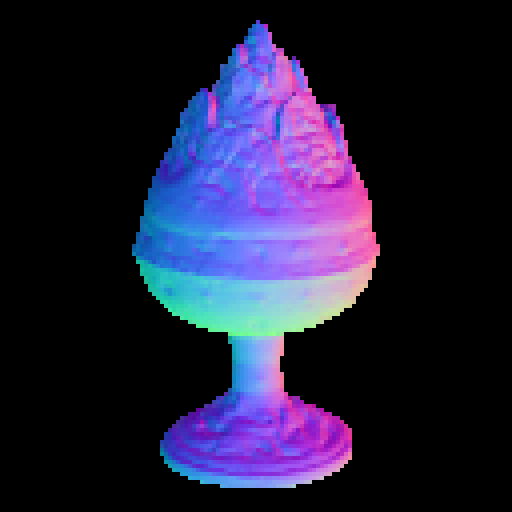
\includegraphics[width=\linewidth]{./Figures/gcnn_synthetic/fancy_eval_2_normal_GCNN-GCNN.png}
	\end{subfigure}
	\begin{subfigure}[b]{0.24\linewidth}
		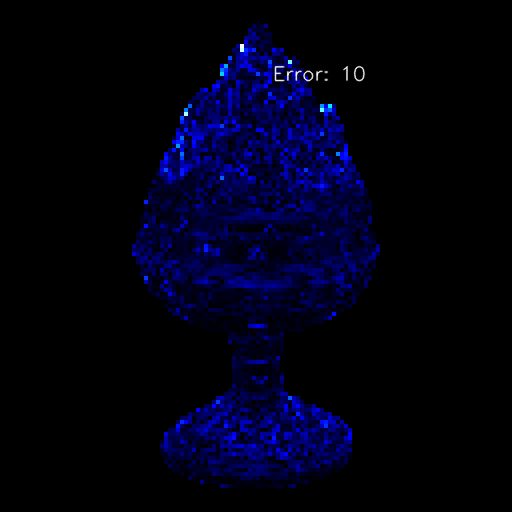
\includegraphics[width=\linewidth]{./Figures/gcnn_synthetic/fancy_eval_2_error_GCNN-GCNN.png}
	\end{subfigure}
	
	
	
	\begin{subfigure}[b]{0.24\linewidth}
		
\includegraphics[width=\linewidth]{./Figures/gcnn_synthetic/eval_2_input.png}
	\end{subfigure}
	\begin{subfigure}[b]{0.24\linewidth}
		
\includegraphics[width=\linewidth]{./Figures/gcnn_synthetic/eval_2_normal_GT.png}
	\end{subfigure}
	\begin{subfigure}[b]{0.24\linewidth}
		
\includegraphics[width=\linewidth]{./Figures/gcnn_synthetic/eval_2_normal_GCNN-GCNN.png}
	\end{subfigure}
	\begin{subfigure}[b]{0.24\linewidth}
		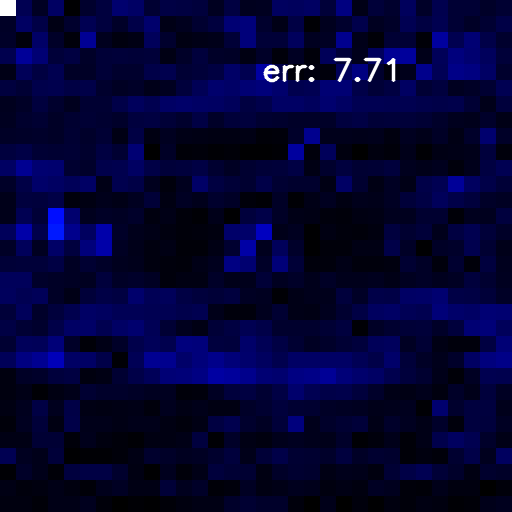
\includegraphics[width=\linewidth]{./Figures/gcnn_synthetic/eval_2_error_GCNN-GCNN.png}
	\end{subfigure}
	
	
	\begin{subfigure}[b]{0.24\linewidth}
		
\includegraphics[width=\linewidth]{./Figures/gcnn_synthetic/fancy_eval_3_point_cloud_noise.png}
	\end{subfigure}
	\begin{subfigure}[b]{0.24\linewidth}
		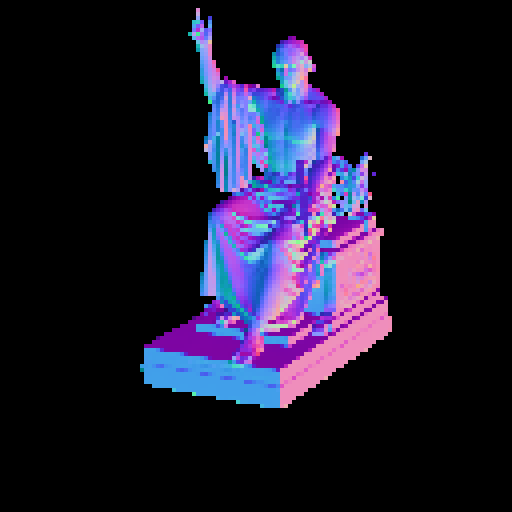
\includegraphics[width=\linewidth]{./Figures/gcnn_synthetic/fancy_eval_3_groundtruth.png}
	\end{subfigure}
	\begin{subfigure}[b]{0.24\linewidth}
		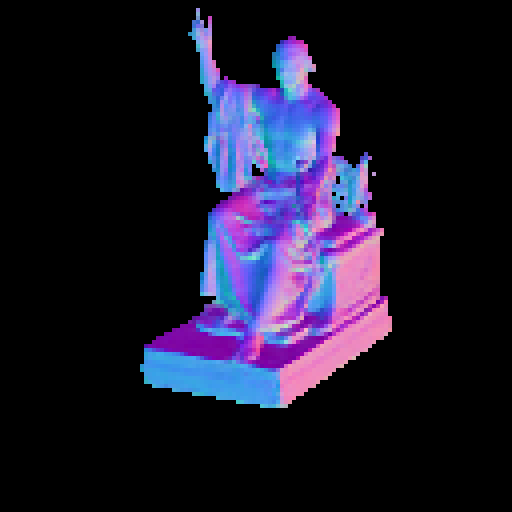
\includegraphics[width=\linewidth]{./Figures/gcnn_synthetic/fancy_eval_3_normal_GCNN-GCNN.png}
	\end{subfigure}
	\begin{subfigure}[b]{0.24\linewidth}
		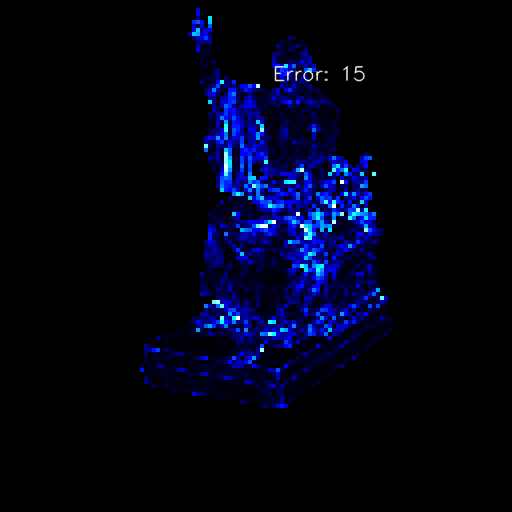
\includegraphics[width=\linewidth]{./Figures/gcnn_synthetic/fancy_eval_3_error_GCNN-GCNN.png}
	\end{subfigure}
	
	
	
	\begin{subfigure}[b]{0.24\linewidth}
		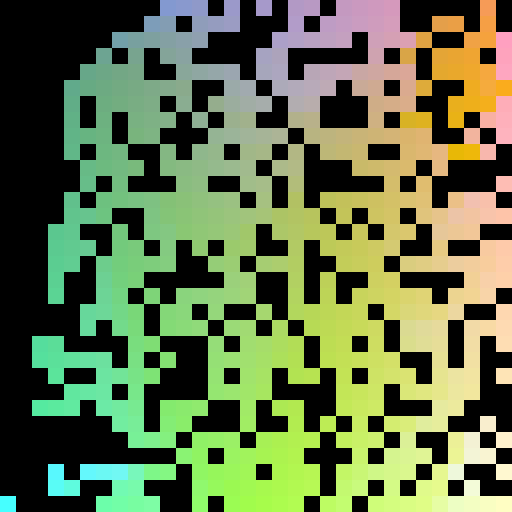
\includegraphics[width=\linewidth]{./Figures/gcnn_synthetic/eval_3_input.png}
	\end{subfigure}
	\begin{subfigure}[b]{0.24\linewidth}
		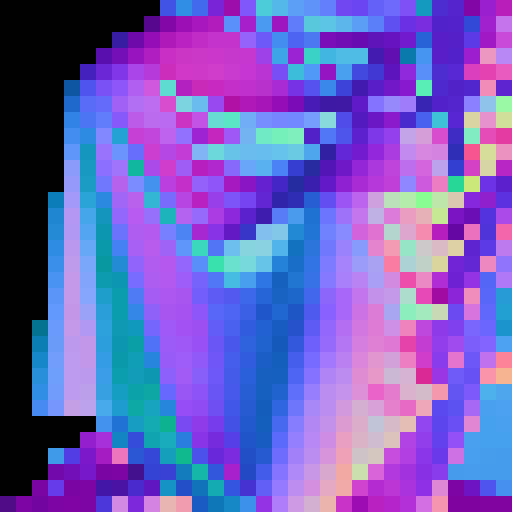
\includegraphics[width=\linewidth]{./Figures/gcnn_synthetic/eval_3_normal_GT.png}
	\end{subfigure}
	\begin{subfigure}[b]{0.24\linewidth}
		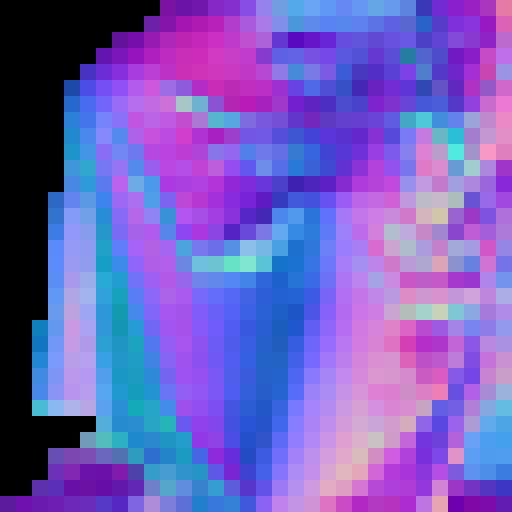
\includegraphics[width=\linewidth]{./Figures/gcnn_synthetic/eval_3_normal_GCNN-GCNN.png}
	\end{subfigure}
	\begin{subfigure}[b]{0.24\linewidth}
		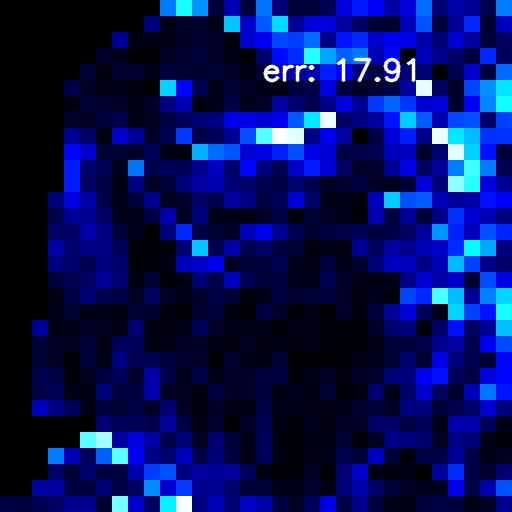
\includegraphics[width=\linewidth]{./Figures/gcnn_synthetic/eval_3_error_GCNN-GCNN.png}
	\end{subfigure}
	
	
	\begin{subfigure}[b]{0.24\linewidth}
		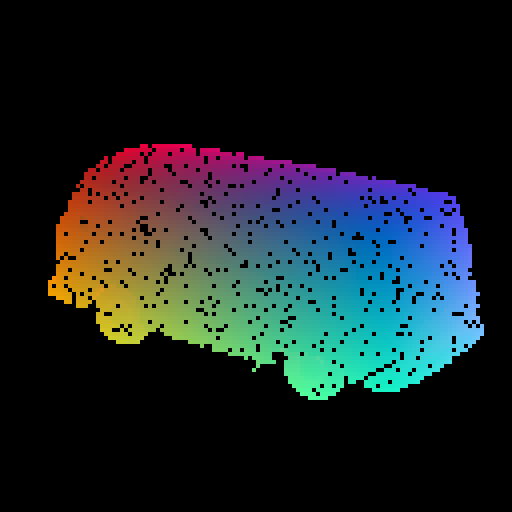
\includegraphics[width=\linewidth]{./Figures/gcnn_synthetic/fancy_eval_9_point_cloud_noise.png}
	\end{subfigure}
	\begin{subfigure}[b]{0.24\linewidth}
		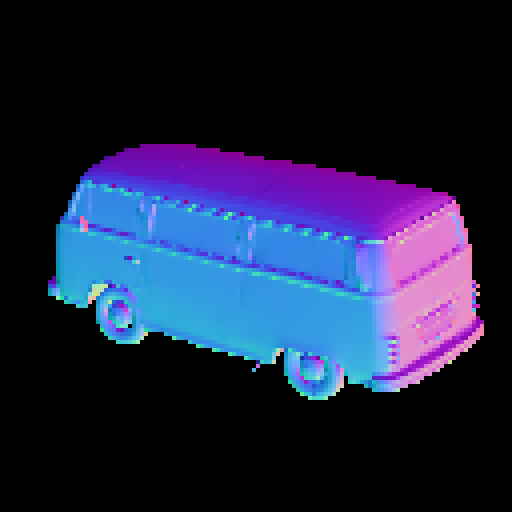
\includegraphics[width=\linewidth]{./Figures/gcnn_synthetic/fancy_eval_9_groundtruth.png}
	\end{subfigure}
	\begin{subfigure}[b]{0.24\linewidth}
		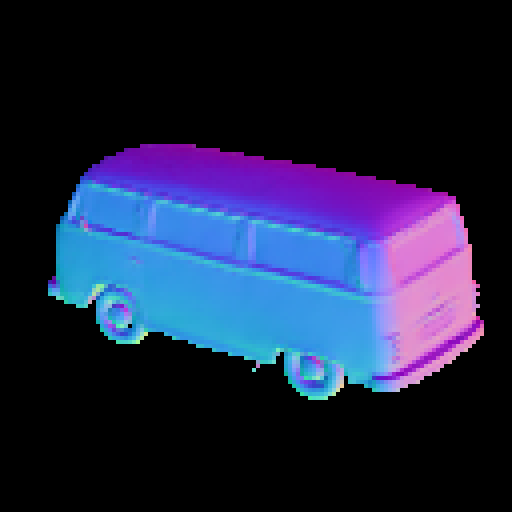
\includegraphics[width=\linewidth]{./Figures/gcnn_synthetic/fancy_eval_9_normal_GCNN-GCNN.png}
	\end{subfigure}
	\begin{subfigure}[b]{0.24\linewidth}
		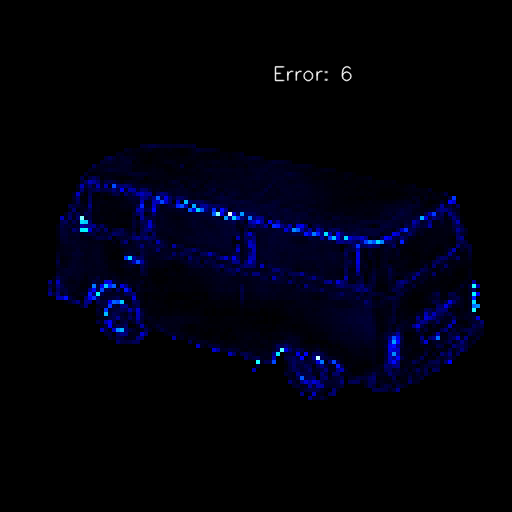
\includegraphics[width=\linewidth]{./Figures/gcnn_synthetic/fancy_eval_9_error_GCNN-GCNN.png}
		
	\end{subfigure}	
	
	\begin{subfigure}[b]{0.24\linewidth}
		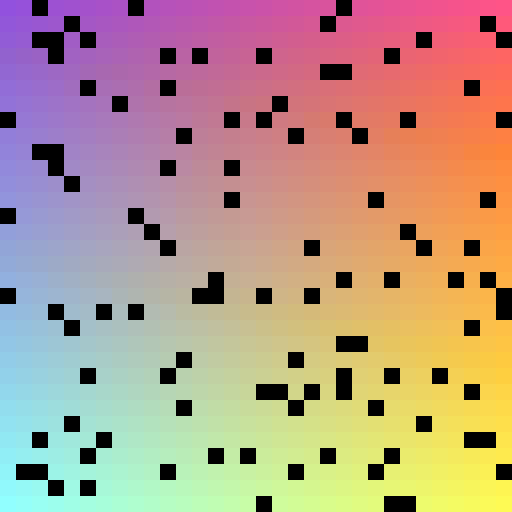
\includegraphics[width=\linewidth]{./Figures/gcnn_synthetic/eval_9_input.png}
		\caption{Vertex}
	\end{subfigure}
	\begin{subfigure}[b]{0.24\linewidth}
		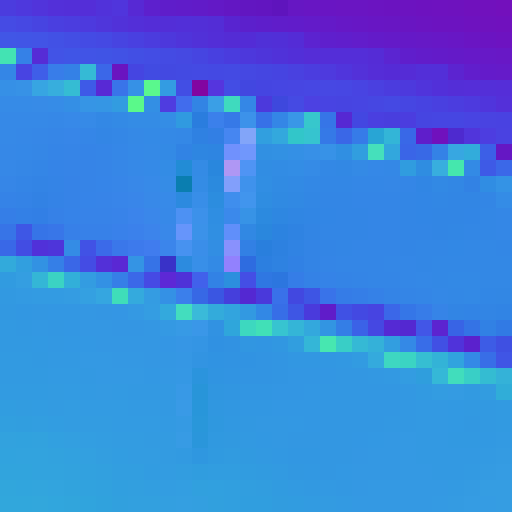
\includegraphics[width=\linewidth]{./Figures/gcnn_synthetic/eval_9_normal_GT.png}
		\caption{GT}
	\end{subfigure}
	\begin{subfigure}[b]{0.24\linewidth}
		
\includegraphics[width=\linewidth]{./Figures/gcnn_synthetic/eval_9_normal_GCNN-GCNN.png}
		\caption{GCNN}
	\end{subfigure}
	\begin{subfigure}[b]{0.24\linewidth}
		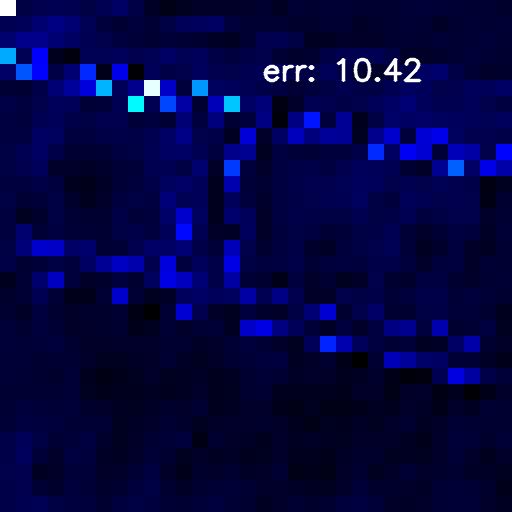
\includegraphics[width=\linewidth]{./Figures/gcnn_synthetic/eval_9_error_GCNN-CNN.png}
		\caption{Error}
	\end{subfigure}
	
	\begin{tikzpicture}
		\node[text width=0.1\textwidth] at (11,-1) {90};
		\node[inner sep=0pt] (input) at (8,-1)
		{
\includegraphics[width=.2\textwidth]{./Figures/colorscale_blue.png}};
		\node[text width=0.3\textwidth] at (7,-1) {Error: 0};
	\end{tikzpicture}
	\decoRule
	\caption{GCNN evaluation ($ 128\times128 $). From top to bottom: Baoshanlu, Washington statue, Bus. }
	\label{fig:gcnn-eval-more}
\end{figure}



%% Trip-Net more evaluation
\begin{figure}
	\centering
	\captionsetup{width=\linewidth}
	\begin{subfigure}[b]{0.19\linewidth}
		
\includegraphics[width=\linewidth]{./Figures/gcnn_synthetic/fancy_eval_2_point_cloud_noise.png}
	\end{subfigure}
	\begin{subfigure}[b]{0.19\linewidth}
	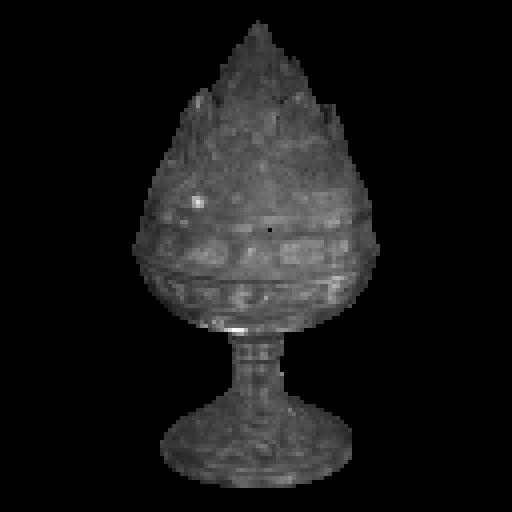
\includegraphics[width=\linewidth]{./Figures/gcnn_synthetic/fancy_eval_2_img.png}
	\end{subfigure}
	\begin{subfigure}[b]{0.19\linewidth}
		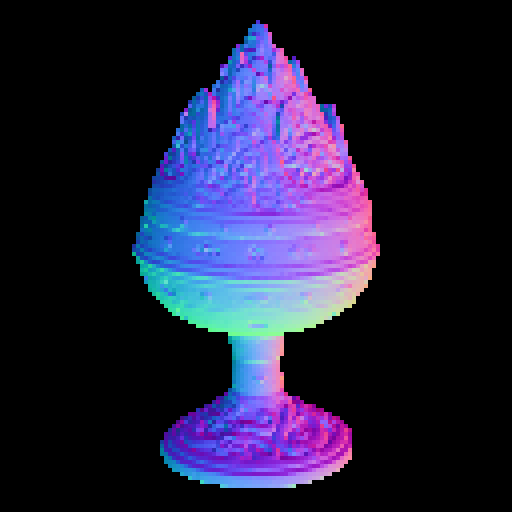
\includegraphics[width=\linewidth]{./Figures/gcnn_synthetic/fancy_eval_2_groundtruth.png}
	\end{subfigure}
	\begin{subfigure}[b]{0.19\linewidth}
		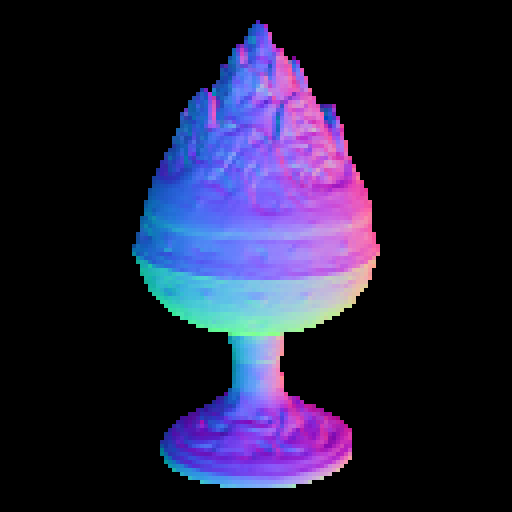
\includegraphics[width=\linewidth]{./Figures/gcnn_synthetic/fancy_eval_2_normal_an2-8-1000.png}
	\end{subfigure}
	\begin{subfigure}[b]{0.19\linewidth}
		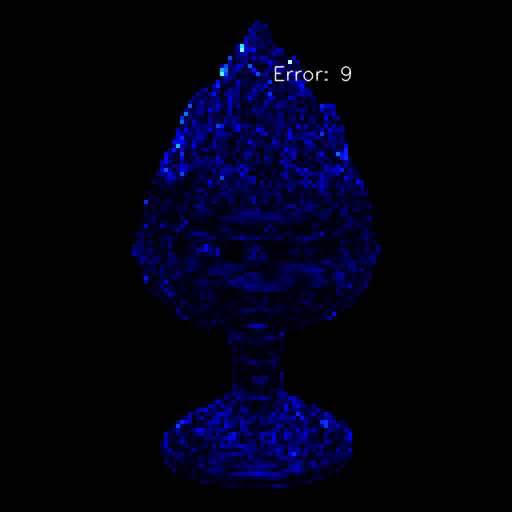
\includegraphics[width=\linewidth]{./Figures/gcnn_synthetic/fancy_eval_2_error_an2-8-1000.png}
	\end{subfigure}
	
	
	
	\begin{subfigure}[b]{0.19\linewidth}
		
\includegraphics[width=\linewidth]{./Figures/gcnn_synthetic/eval_2_input.png}
	\end{subfigure}
	\begin{subfigure}[b]{0.19\linewidth}
	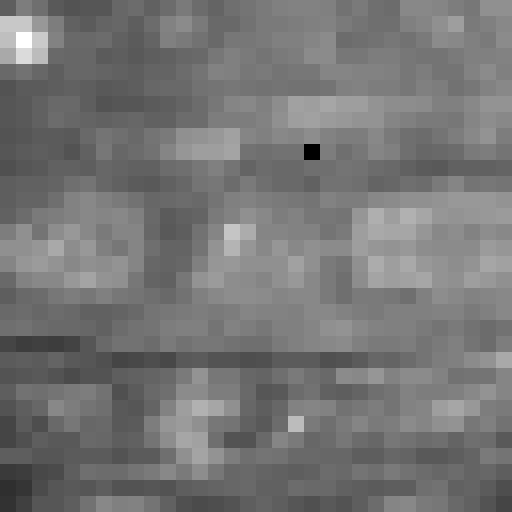
\includegraphics[width=\linewidth]{./Figures/gcnn_synthetic/eval_2_img.png}
	\end{subfigure}
	\begin{subfigure}[b]{0.19\linewidth}
		
\includegraphics[width=\linewidth]{./Figures/gcnn_synthetic/eval_2_normal_GT.png}
	\end{subfigure}
	\begin{subfigure}[b]{0.19\linewidth}
		
\includegraphics[width=\linewidth]{./Figures/gcnn_synthetic/eval_2_normal_an2-8-1000.png}
	\end{subfigure}
	\begin{subfigure}[b]{0.19\linewidth}
		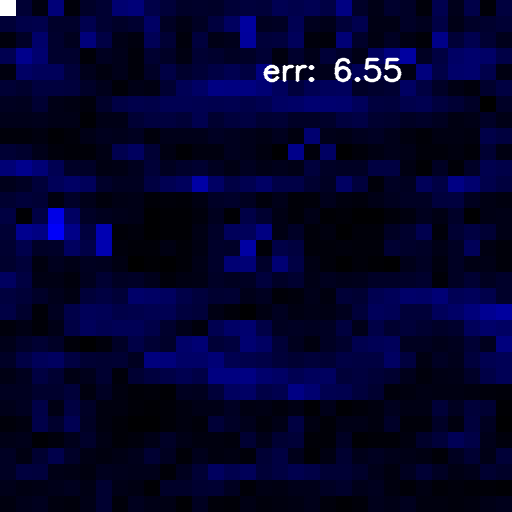
\includegraphics[width=\linewidth]{./Figures/gcnn_synthetic/eval_2_error_an2-8-1000.png}
	\end{subfigure}
	
	
	\begin{subfigure}[b]{0.19\linewidth}
		
\includegraphics[width=\linewidth]{./Figures/gcnn_synthetic/fancy_eval_3_point_cloud_noise.png}
	\end{subfigure}
	\begin{subfigure}[b]{0.19\linewidth}
	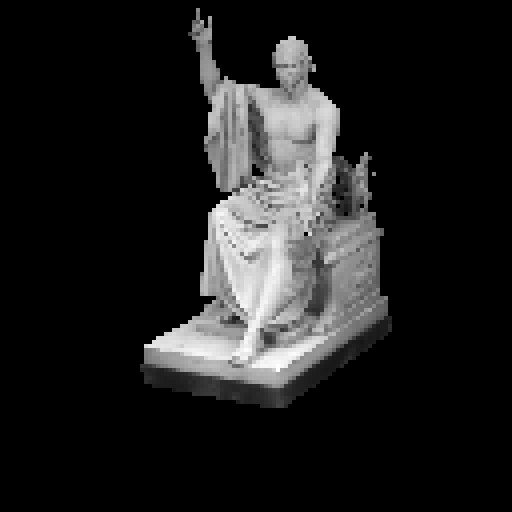
\includegraphics[width=\linewidth]{./Figures/gcnn_synthetic/fancy_eval_3_img.png}
\end{subfigure}
	\begin{subfigure}[b]{0.19\linewidth}
		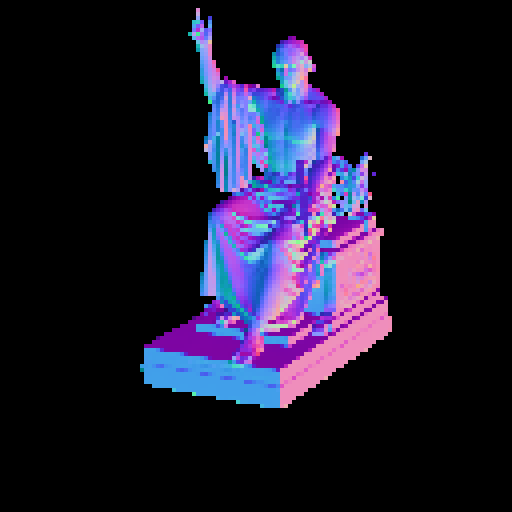
\includegraphics[width=\linewidth]{./Figures/gcnn_synthetic/fancy_eval_3_groundtruth.png}
	\end{subfigure}
	\begin{subfigure}[b]{0.19\linewidth}
		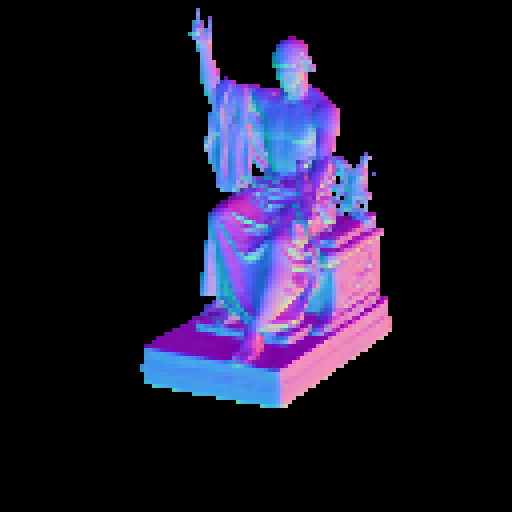
\includegraphics[width=\linewidth]{./Figures/gcnn_synthetic/fancy_eval_3_normal_an2-8-1000.png}
	\end{subfigure}
	\begin{subfigure}[b]{0.19\linewidth}
		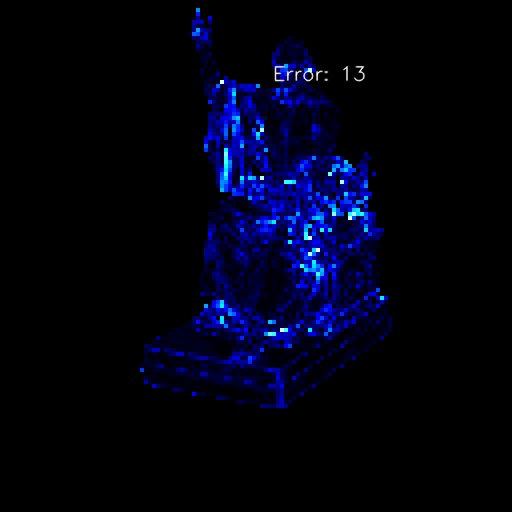
\includegraphics[width=\linewidth]{./Figures/gcnn_synthetic/fancy_eval_3_error_an2-8-1000.png}
	\end{subfigure}
	
	
	
	\begin{subfigure}[b]{0.19\linewidth}
		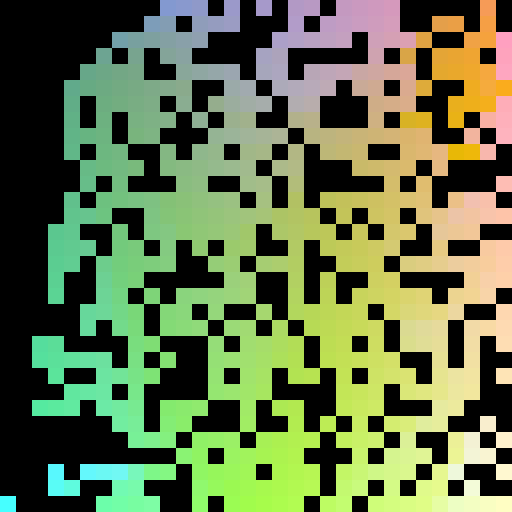
\includegraphics[width=\linewidth]{./Figures/gcnn_synthetic/eval_3_input.png}
	\end{subfigure}
	\begin{subfigure}[b]{0.19\linewidth}
	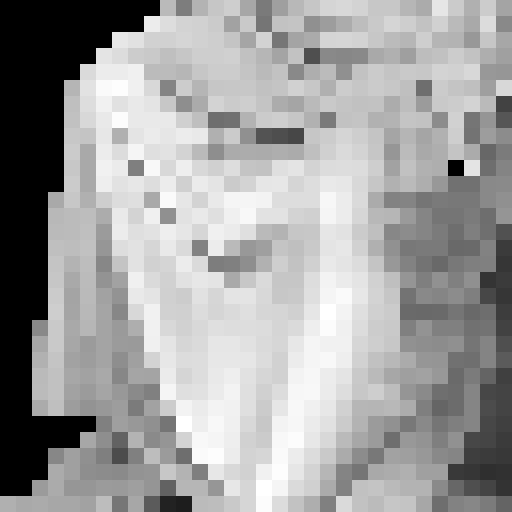
\includegraphics[width=\linewidth]{./Figures/gcnn_synthetic/eval_3_img.png}
	\end{subfigure}
	\begin{subfigure}[b]{0.19\linewidth}
		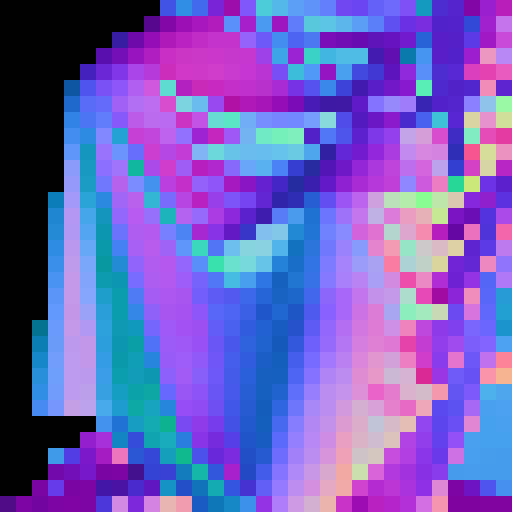
\includegraphics[width=\linewidth]{./Figures/gcnn_synthetic/eval_3_normal_GT.png}
	\end{subfigure}
	\begin{subfigure}[b]{0.19\linewidth}
		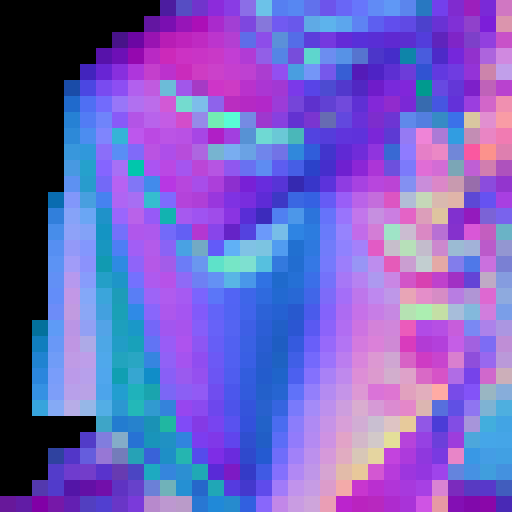
\includegraphics[width=\linewidth]{./Figures/gcnn_synthetic/eval_3_normal_an2-8-1000.png}
	\end{subfigure}
	\begin{subfigure}[b]{0.19\linewidth}
		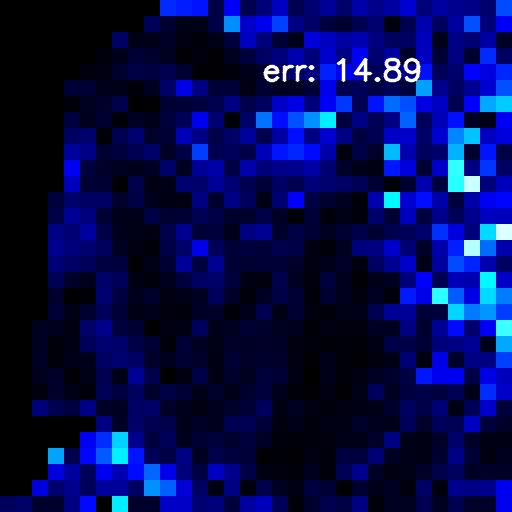
\includegraphics[width=\linewidth]{./Figures/gcnn_synthetic/eval_3_error_an2-8-1000.png}
	\end{subfigure}
	
	
	\begin{subfigure}[b]{0.19\linewidth}
		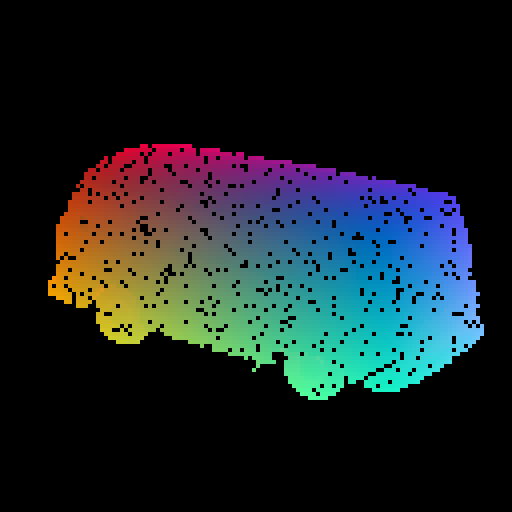
\includegraphics[width=\linewidth]{./Figures/gcnn_synthetic/fancy_eval_9_point_cloud_noise.png}
	\end{subfigure}
	\begin{subfigure}[b]{0.19\linewidth}
	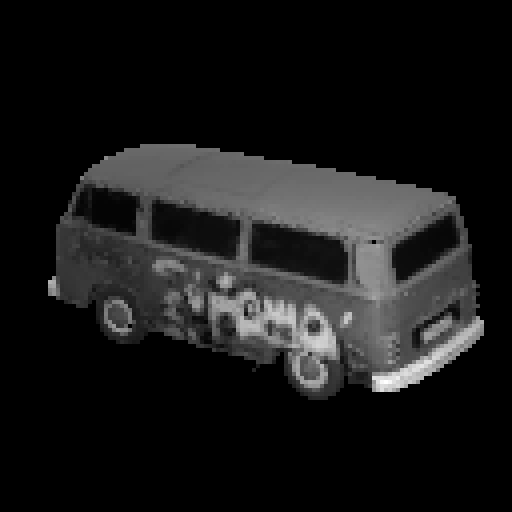
\includegraphics[width=\linewidth]{./Figures/gcnn_synthetic/fancy_eval_9_img.png}
	\end{subfigure}
	\begin{subfigure}[b]{0.19\linewidth}
		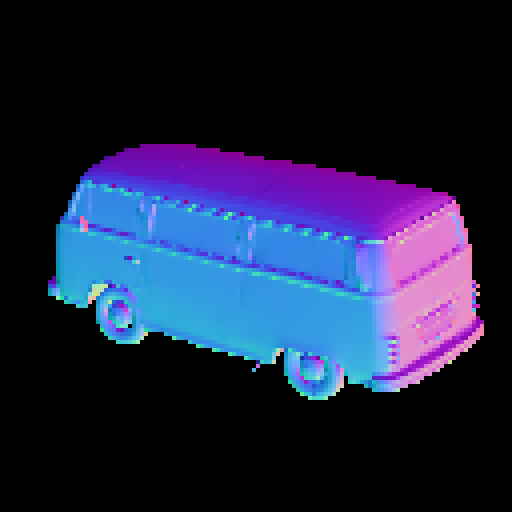
\includegraphics[width=\linewidth]{./Figures/gcnn_synthetic/fancy_eval_9_groundtruth.png}
	\end{subfigure}
	\begin{subfigure}[b]{0.19\linewidth}
		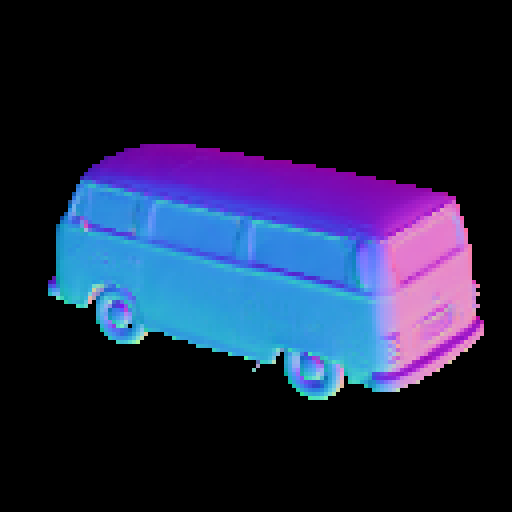
\includegraphics[width=\linewidth]{./Figures/gcnn_synthetic/fancy_eval_9_normal_an2-8-1000.png}
	\end{subfigure}
	\begin{subfigure}[b]{0.19\linewidth}
		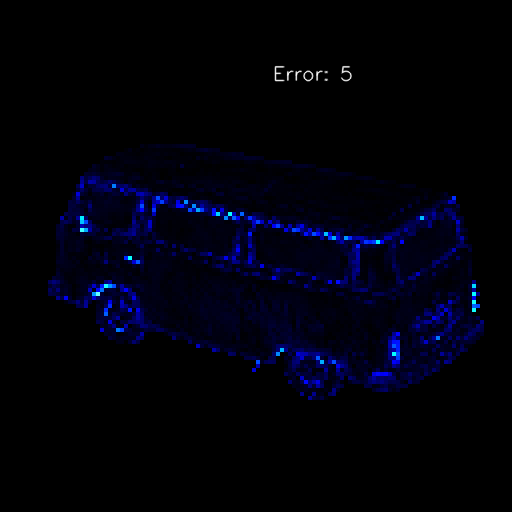
\includegraphics[width=\linewidth]{./Figures/gcnn_synthetic/fancy_eval_9_error_an2-8-1000.png}
	\end{subfigure}	
	
	\begin{subfigure}[b]{0.19\linewidth}
		\includegraphics[width=\linewidth]{./Figures/gcnn_synthetic/eval_9_input.png}
		\caption{Vertex}
	\end{subfigure}
	\begin{subfigure}[b]{0.19\linewidth}
	\includegraphics[width=\linewidth]{./Figures/gcnn_synthetic/eval_9_img.png}
	\caption{Image}
	\end{subfigure}
	\begin{subfigure}[b]{0.19\linewidth}
		\includegraphics[width=\linewidth]{./Figures/gcnn_synthetic/eval_9_normal_GT.png}
		\caption{GT}
	\end{subfigure}
	\begin{subfigure}[b]{0.19\linewidth}
		\includegraphics[width=\linewidth]{./Figures/gcnn_synthetic/eval_9_normal_an2-8-1000.png}
		\caption{Trip-Net}
	\end{subfigure}
	\begin{subfigure}[b]{0.19\linewidth}
		\includegraphics[width=\linewidth]{./Figures/gcnn_synthetic/eval_9_error_an2-8-1000.png}
		\caption{Error}
	\end{subfigure}
	
	
	
	
	\begin{tikzpicture}
		\node[text width=0.1\textwidth] at (11,-1) {90};
		\node[inner sep=0pt] (input) at (8,-1)
		{\includegraphics[width=.2\textwidth]{./Figures/colorscale_blue.png}};
		\node[text width=0.3\textwidth] at (7,-1) {Error: 0};
	\end{tikzpicture}
	\decoRule
	\caption{Trip-Net evaluation ($ 128\times 128 $). From top to bottom: Baoshanlu, Washington statue, Bus.}
	\label{fig:trip-net-eval-more}
\end{figure}
